\section{Initial volume}
 \begin{figure}[H]
  \centering
  \captionsetup{width=.8\linewidth} 
  \includegraphics[width=1\textwidth]
  {{images/8_workflow6_InitialVolume.pdf}}
  \caption{Initial volume (Purple color).}
  \label{fig:workflow_6}
  \end{figure}

Right angles of each projection image are needed to reconstruct the \ttt{3D} map. In \ttt{3D EM}, however, these angles are unknown and we have to estimate them. The most popular way of estimating them is comparing the projections of a  volume similar to ours, known as initial volume, with the images obtained from the microscope. Since the 3D map reconstruction process requires an approximate low resolution map to be refined in further steps according to the projection images of particles, in this tutorial we are going to generate a $de-novo$ initial map model combining the results obtained by different algorithms: First, to compute the initial volume using the set of aligned particles as input, we have used $cryoSPARC$ \ttt{Stochastic Gradient Descent (SGD)} and $Relion$ \ttt{Stochastic Gradient Descent (SGD)} (\ffigure{fig:workflow_6}, left). Second, to generate the initial volume from the class representative particles, we have run $Xmipp$ \ttt{reconstruct significant} and $Xmipp$ \ttt{RANSAC} (\ffigure{fig:workflow_6}, right). $Xmipp$ \ttt{reconstruct significant} sets the map in a \ttt{Weighted Least Square} framework and calculates weights through a statistical approach based on the cumulative density function of different image similarity measures. $Xmipp$ \ttt{RANSAC} is based on an initial non-lineal dimension reduction approach with which selecting sets of class representative images that capture the most of the structural information of each particle. These reduced sets will be used to build maps starting from random orientation assignments. The best map will be selected from these previous assumptions using a random sample consensus (RANSAC) approach.

\subsection*{$cryoSPARC$ \ttt{Stochastic Gradient Descent (SGD)}}
The algorithm $cryoSPARC$ \ttt{Stochastic Gradient Descent (SGD)} has been implemented in the protocol \scommand{cryosparc2-initial model} (\ffigure{fig:initial_vol_1}). The set of particles selected in the previous step is used as input (see the \ttt{Input} tap of the protocol form). 

\begin{figure}[H]
  \centering
  \captionsetup{width=.8\linewidth} 
  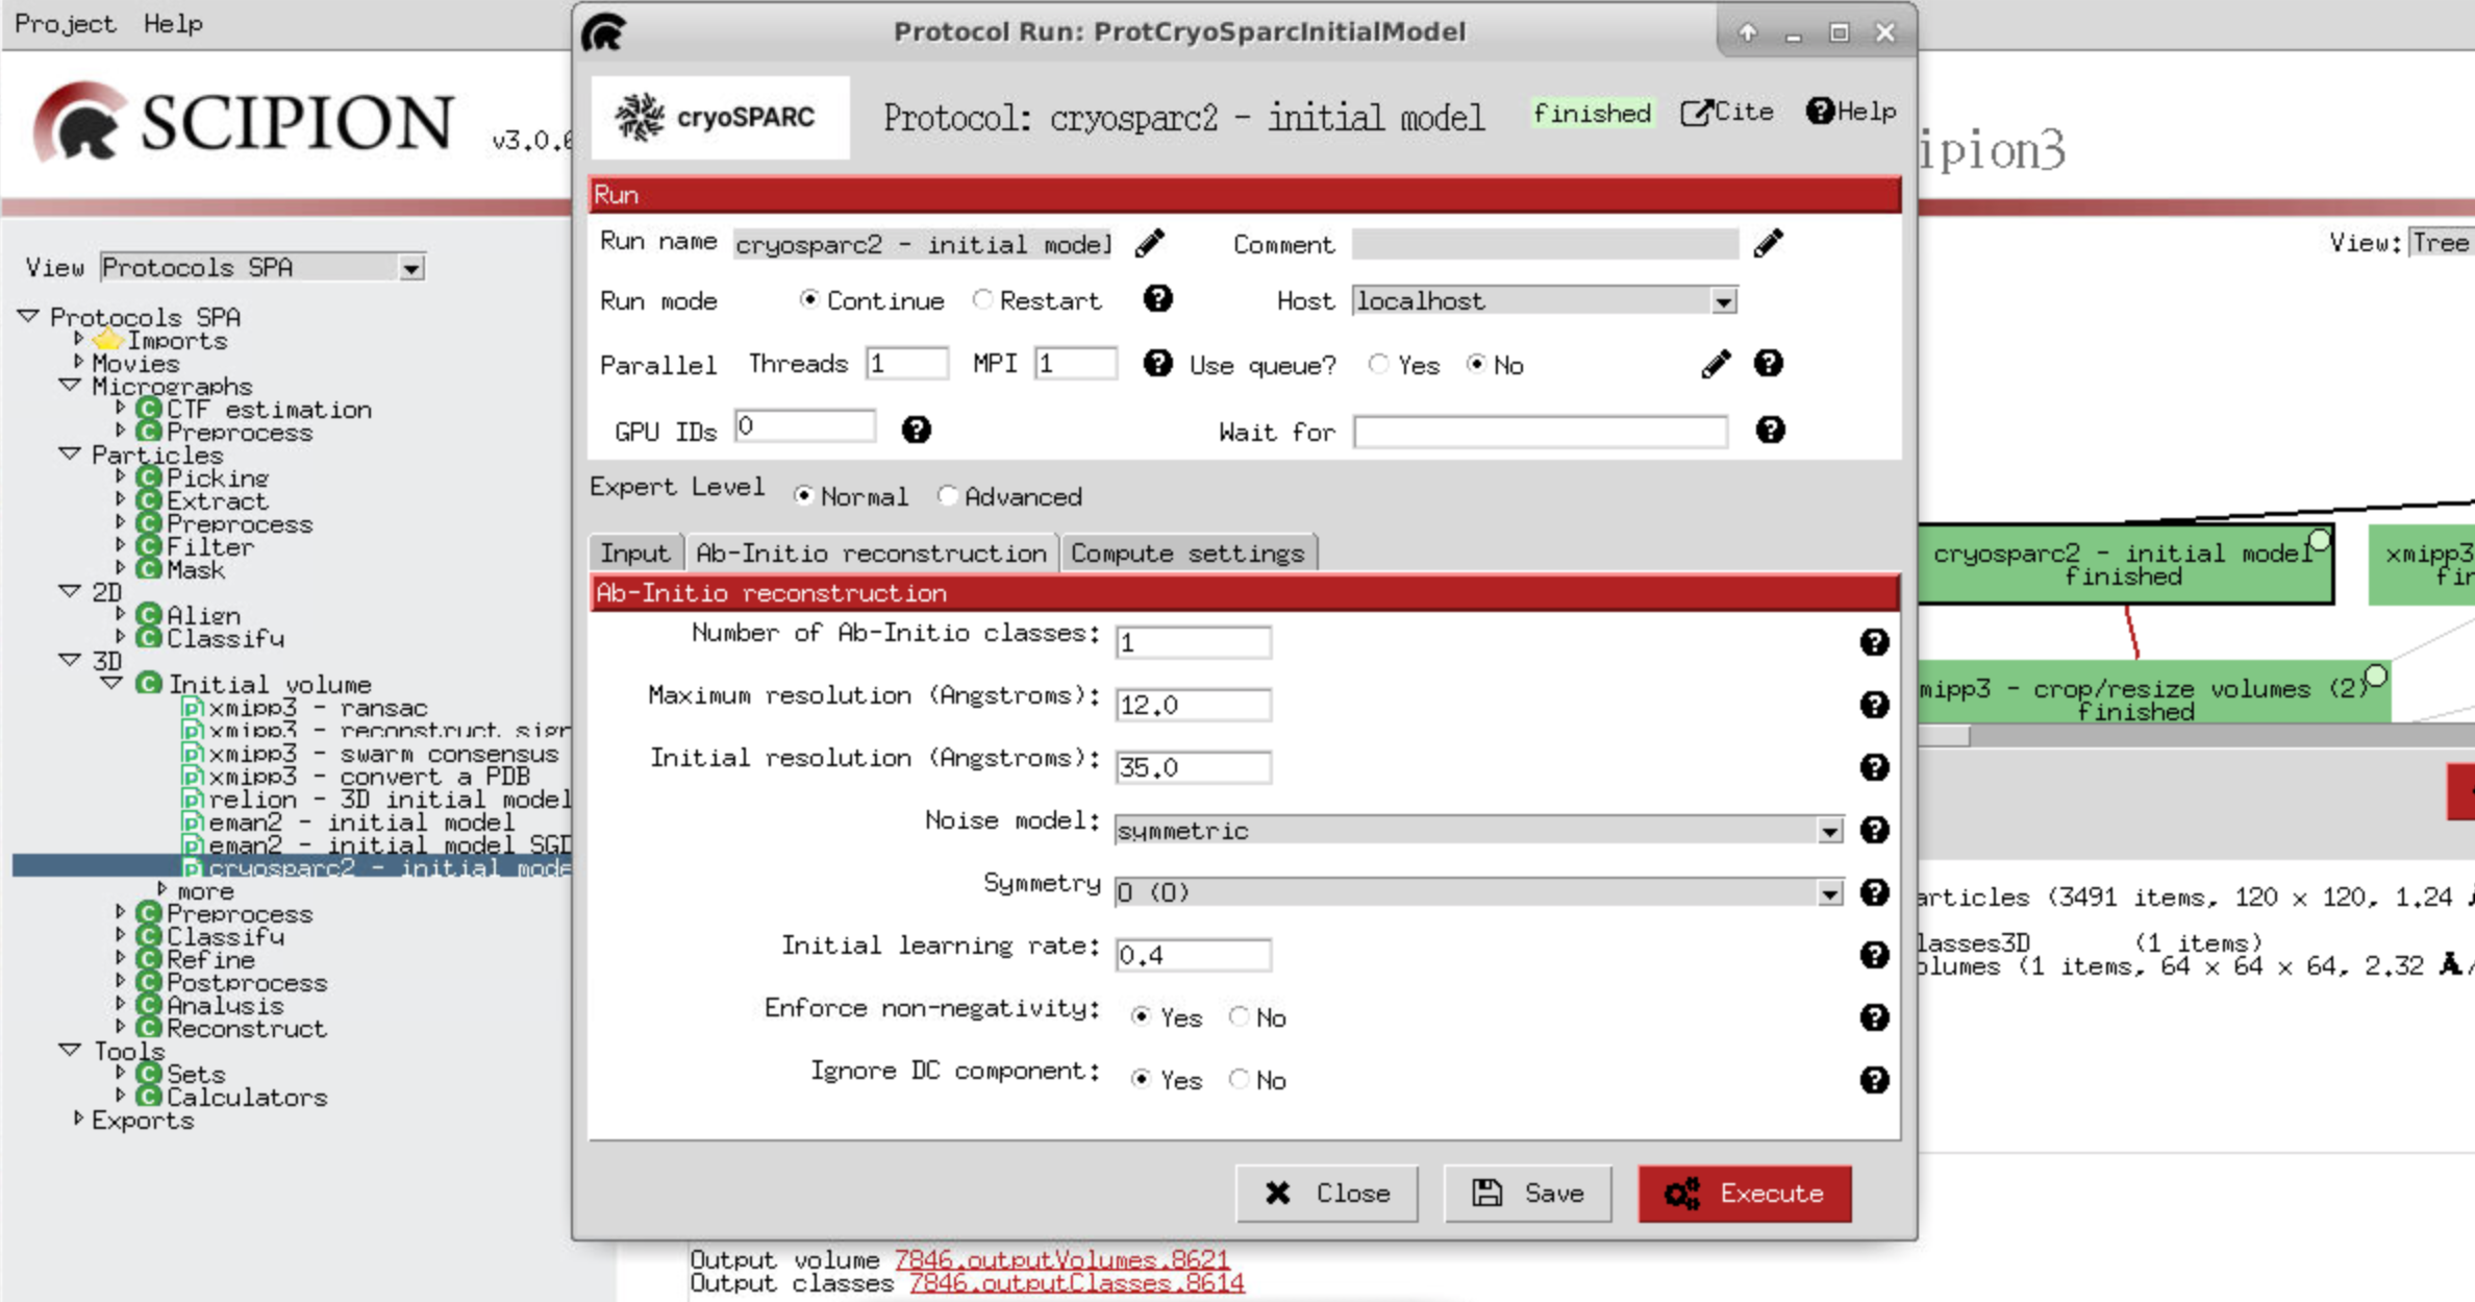
\includegraphics[width=0.95\textwidth]
  {images/8a_cryosparc2_initialmodel.pdf}
  \caption{Completing the second tap of the protocol \scommand{cryosparc2-initial model} with one \ttt{Ab-Initio} class and octahedral \ttt{Symmetry}.}
  \label{fig:initial_vol_1}
  \end{figure}
  
In this case, only one \ttt{Ab-Initio} class has been selected and octahedral \ttt{Symmetry} has been considered (\ffigure{fig:initial_vol_1}). The \ttt{Ab-Initio} class will be randomly initialized, unless an initial map is provided. In that case, the class will be a random variant of the initial map. Regarding symmetries, enforcing symmetry above C1 is not recommendable for $ab-initio$ reconstructions. The volume or the \ttt{3D} class generated can be appreciated by pressing \scommand{Analyze Results}.\\

Since the size and sampling rate of maps generated with \scommand{cryosparc2-initial model} differ from the size and sampling rate of the input particles, a resizing intermediate method has to be applied to recover these dimensions. Protocol \scommand{xmipp3-crop/resize volumes} will help us with this task (\ffigure{fig:crop_resize}). As input, select the output volume\/s of the previous protocols, \ttt{Sampling Rate} for \ttt{Resize option}, and 120 pixels as \ttt{New image size}.

\begin{figure}[H]
  \centering
  \captionsetup{width=.8\linewidth} 
  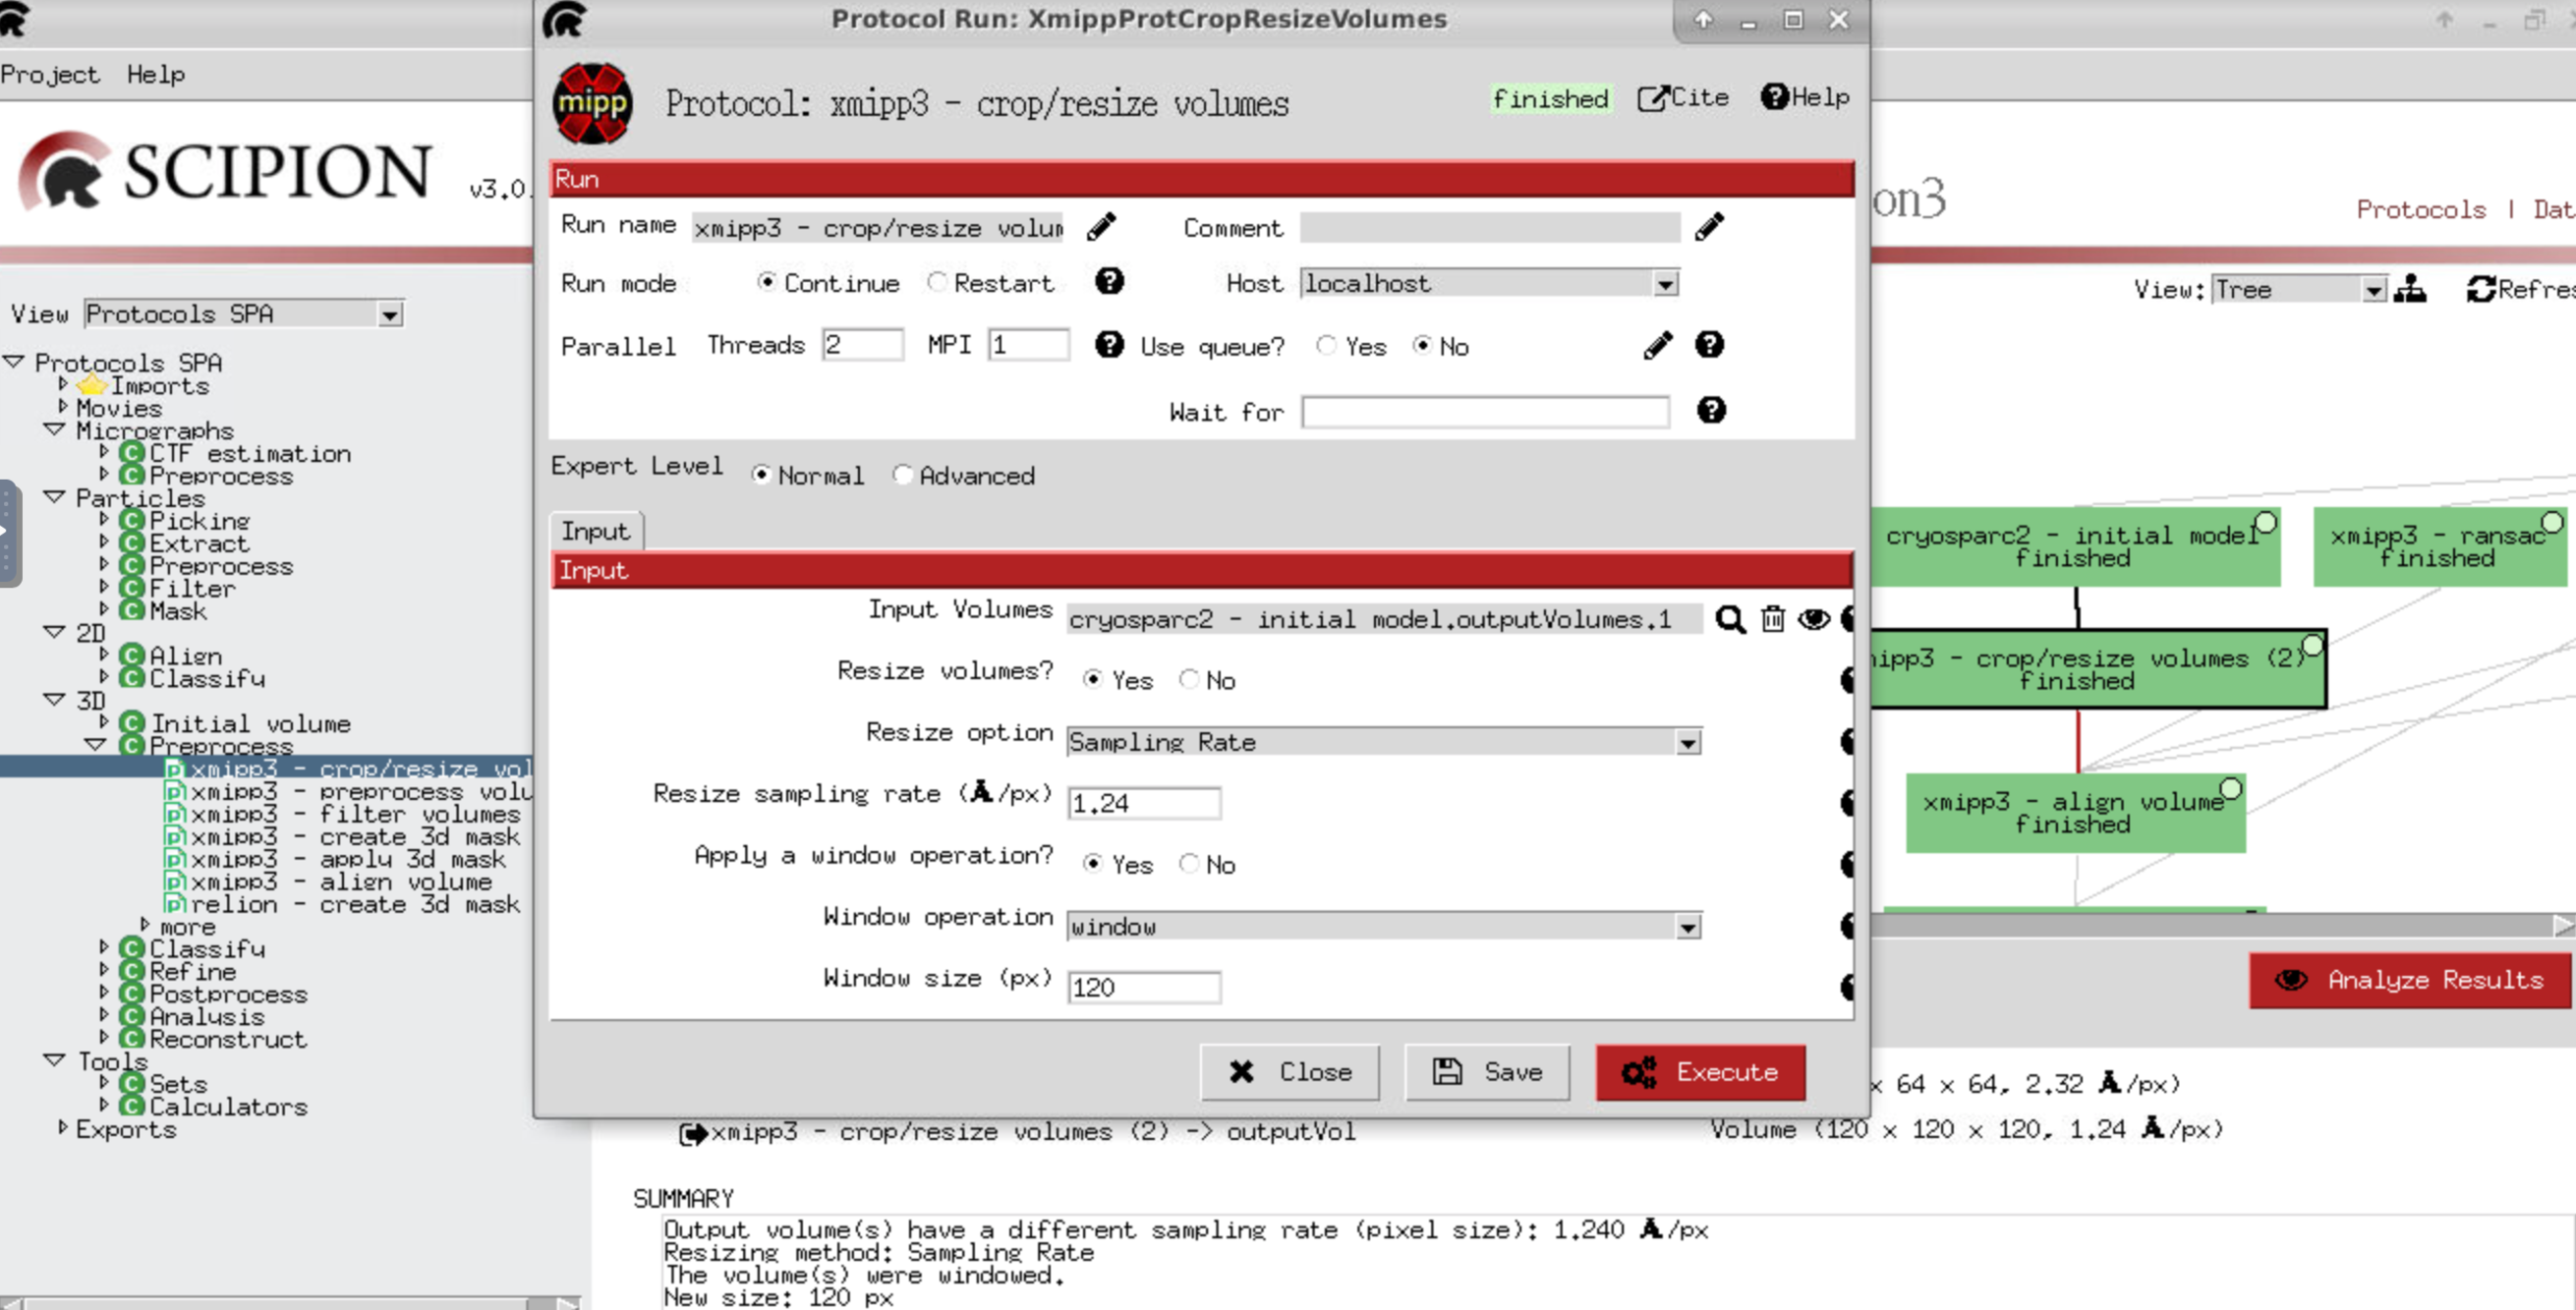
\includegraphics[width=0.95\textwidth]
  {images/8e_xmipp3_cropRS.pdf}
  \caption{Completing the protocol \scommand{xmipp3-crop/resize volumes}.}
  \label{fig:crop_resize}
  \end{figure}

\subsection*{$Relion$ \ttt{Stochastic Gradient Descent (SGD)}}
$Relion$ \ttt{Stochastic Gradient Descent (SGD)} has been implemented in the protocol \scommand{relion-3D initial model}. As input we are using the same set of particles as $cryoSPARC$ \ttt{Stochastic Gradient Descent (SGD)}. And to fill in the param values we used one \ttt{class} and octahedral \ttt{Symmetry} and we executed it (\ffigure{fig:initial_vol_2}). 

\begin{figure}[H]
  \centering
  \captionsetup{width=.8\linewidth} 
  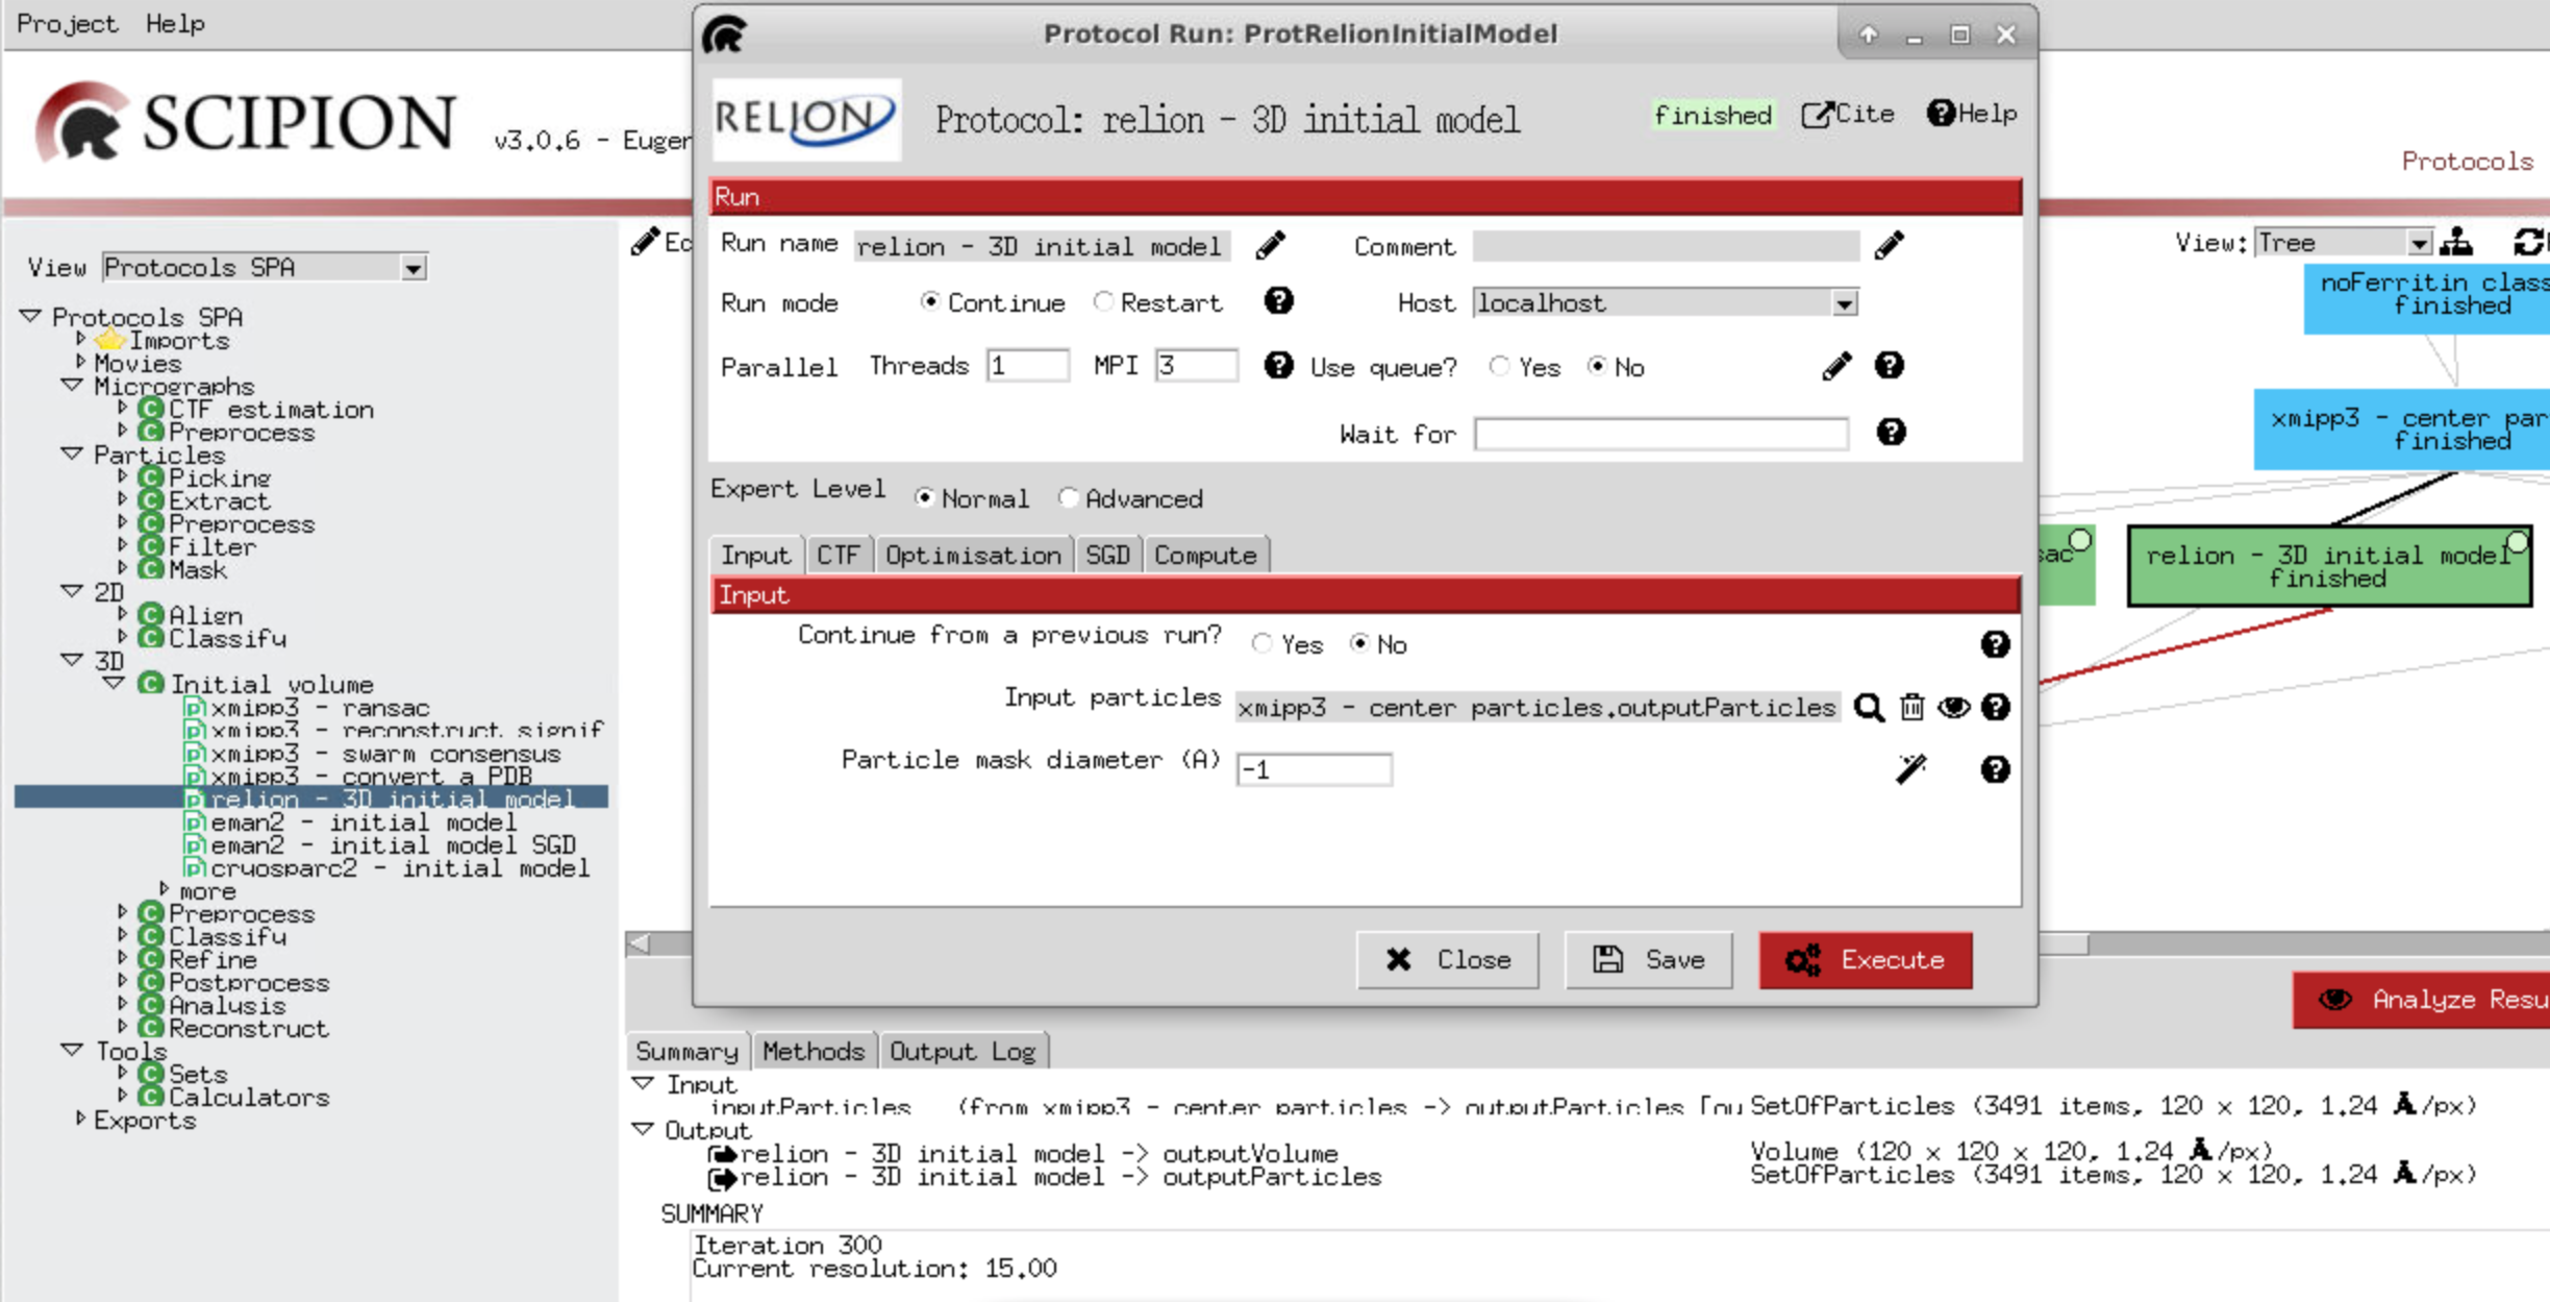
\includegraphics[width=0.95\textwidth]
  {images/8c_relion3DInitialModel.pdf}
  \caption{Filling in the \ttt{Input} tap of the protocol \scommand{relion-3D initial model}.}
  \label{fig:initial_vol_2}
  \end{figure}

  Only one volume has been generated with this protocol that keeps size and sampling rate of the input particles. You can visualize it with \chimera in 3D by pressing \scommand{Analyze Results} and selecting in the \ttt{Volumes} box \ttt{Display volume with} \ttt{chimera}. 
  
\subsection*{$Xmipp$}
Using the 38 class representative particles as input, as well as the type of symmetry (octahedral), the protocol \scommand{xmipp3-reconstruct significant} (\ffigure{fig:xmipp_reconstruct_significant}) also generates one initial volume and preserves the size and sampling rate of the input \ttt{2D} classes.

\begin{figure}[H]
  \centering
  \captionsetup{width=.8\linewidth} 
  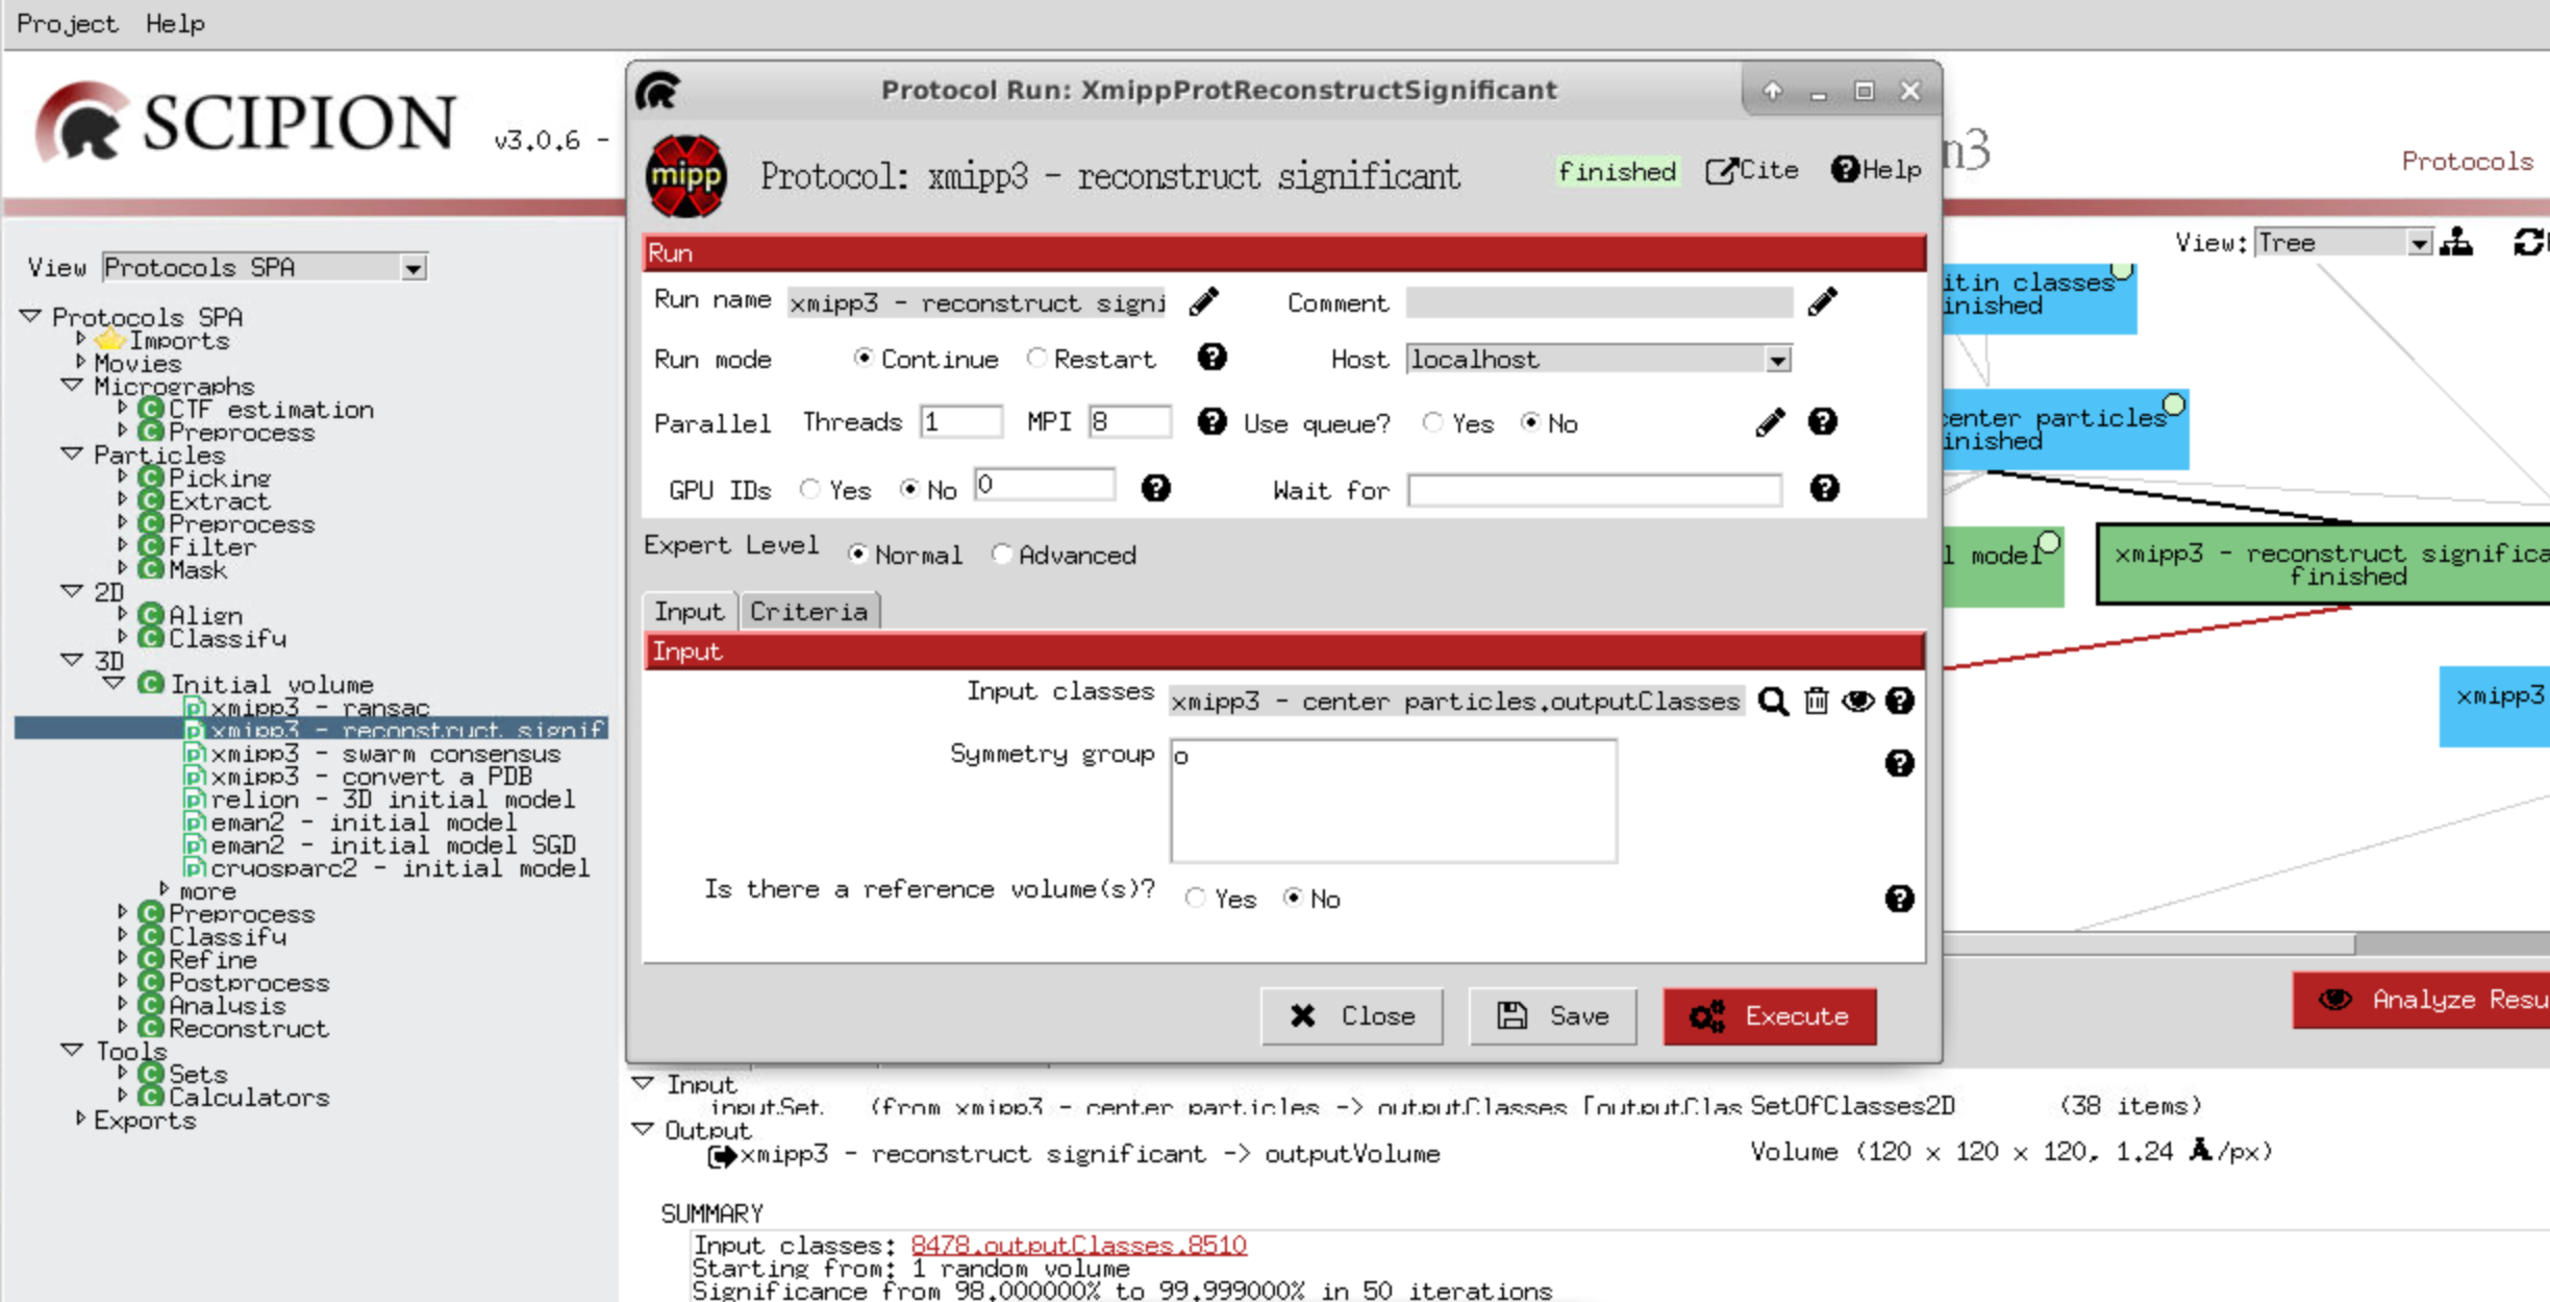
\includegraphics[width=0.95\textwidth]
  {images/8d_xmipp3_reconstructSig.pdf}
  \caption{Completing the \ttt{Input} tap of the protocol \scommand{xmipp3-reconstruct significant}.}
  \label{fig:xmipp_reconstruct_significant}
  \end{figure}

$Xmipp$ \ttt{RANSAC} algorithm, implemented in the protocol \scommand{xmipp3-ransac} (\ffigure{fig:xmipp_ransac}), although starts from the same input than $Xmipp$ \ttt{reconstruct significant}, generates 10 different maps and preserves the size and sampling rate from the input \ttt{2D} classes. You can choose a different number of output maps in the advanced param \ttt{Number of best volumes to refine}.

\begin{figure}[H]
  \centering
  \captionsetup{width=.8\linewidth} 
  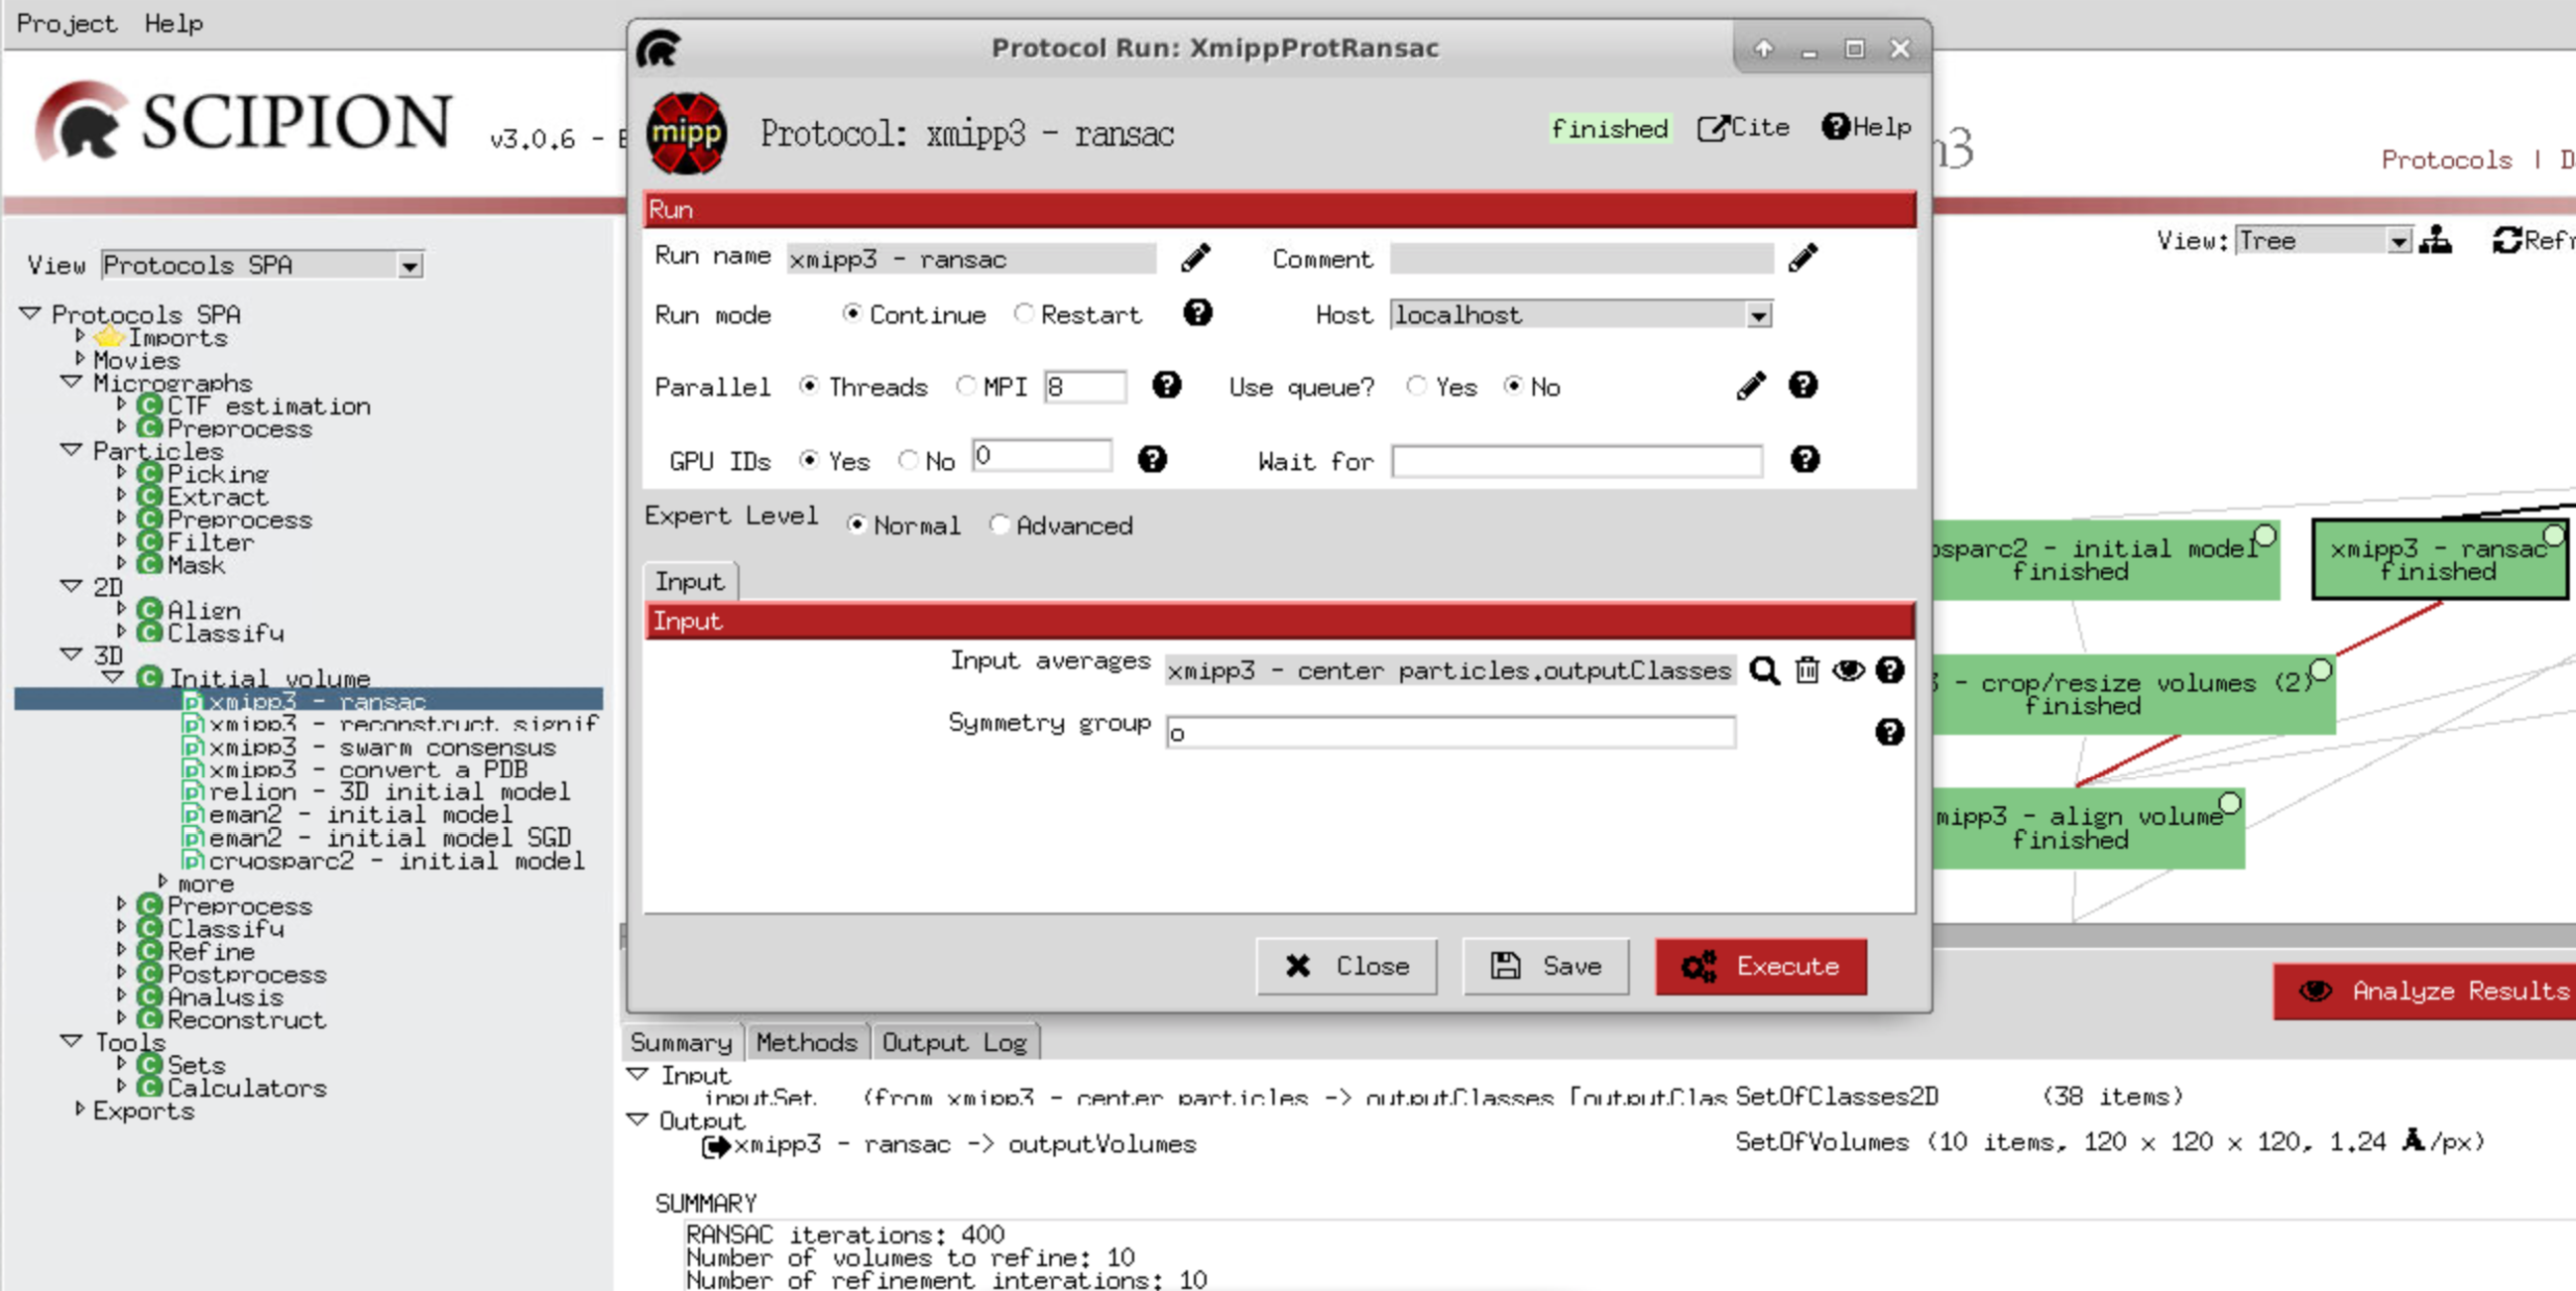
\includegraphics[width=0.95\textwidth]
  {images/8b_xmipp3_ransac.pdf}
  \caption{Filling in the params of the protocol \scommand{xmipp3-ransac}.}
  \label{fig:xmipp_ransac}
  \end{figure}
  
\subsection*{Map alignment and swarm consensus}
Next, we perform a fast fourier alignment of the 13 maps (volumes) generated, starting both from particles and \ttt{2D} classes, using the protocol \scommand{xmipp3-align volume} (\ffigure{fig:align_volume}). As \ttt{Reference volume} we select the initial volume obtained by the $Xmipp$ reconstruct significant algorithm.

\begin{figure}[H]
  \centering
  \captionsetup{width=.8\linewidth} 
  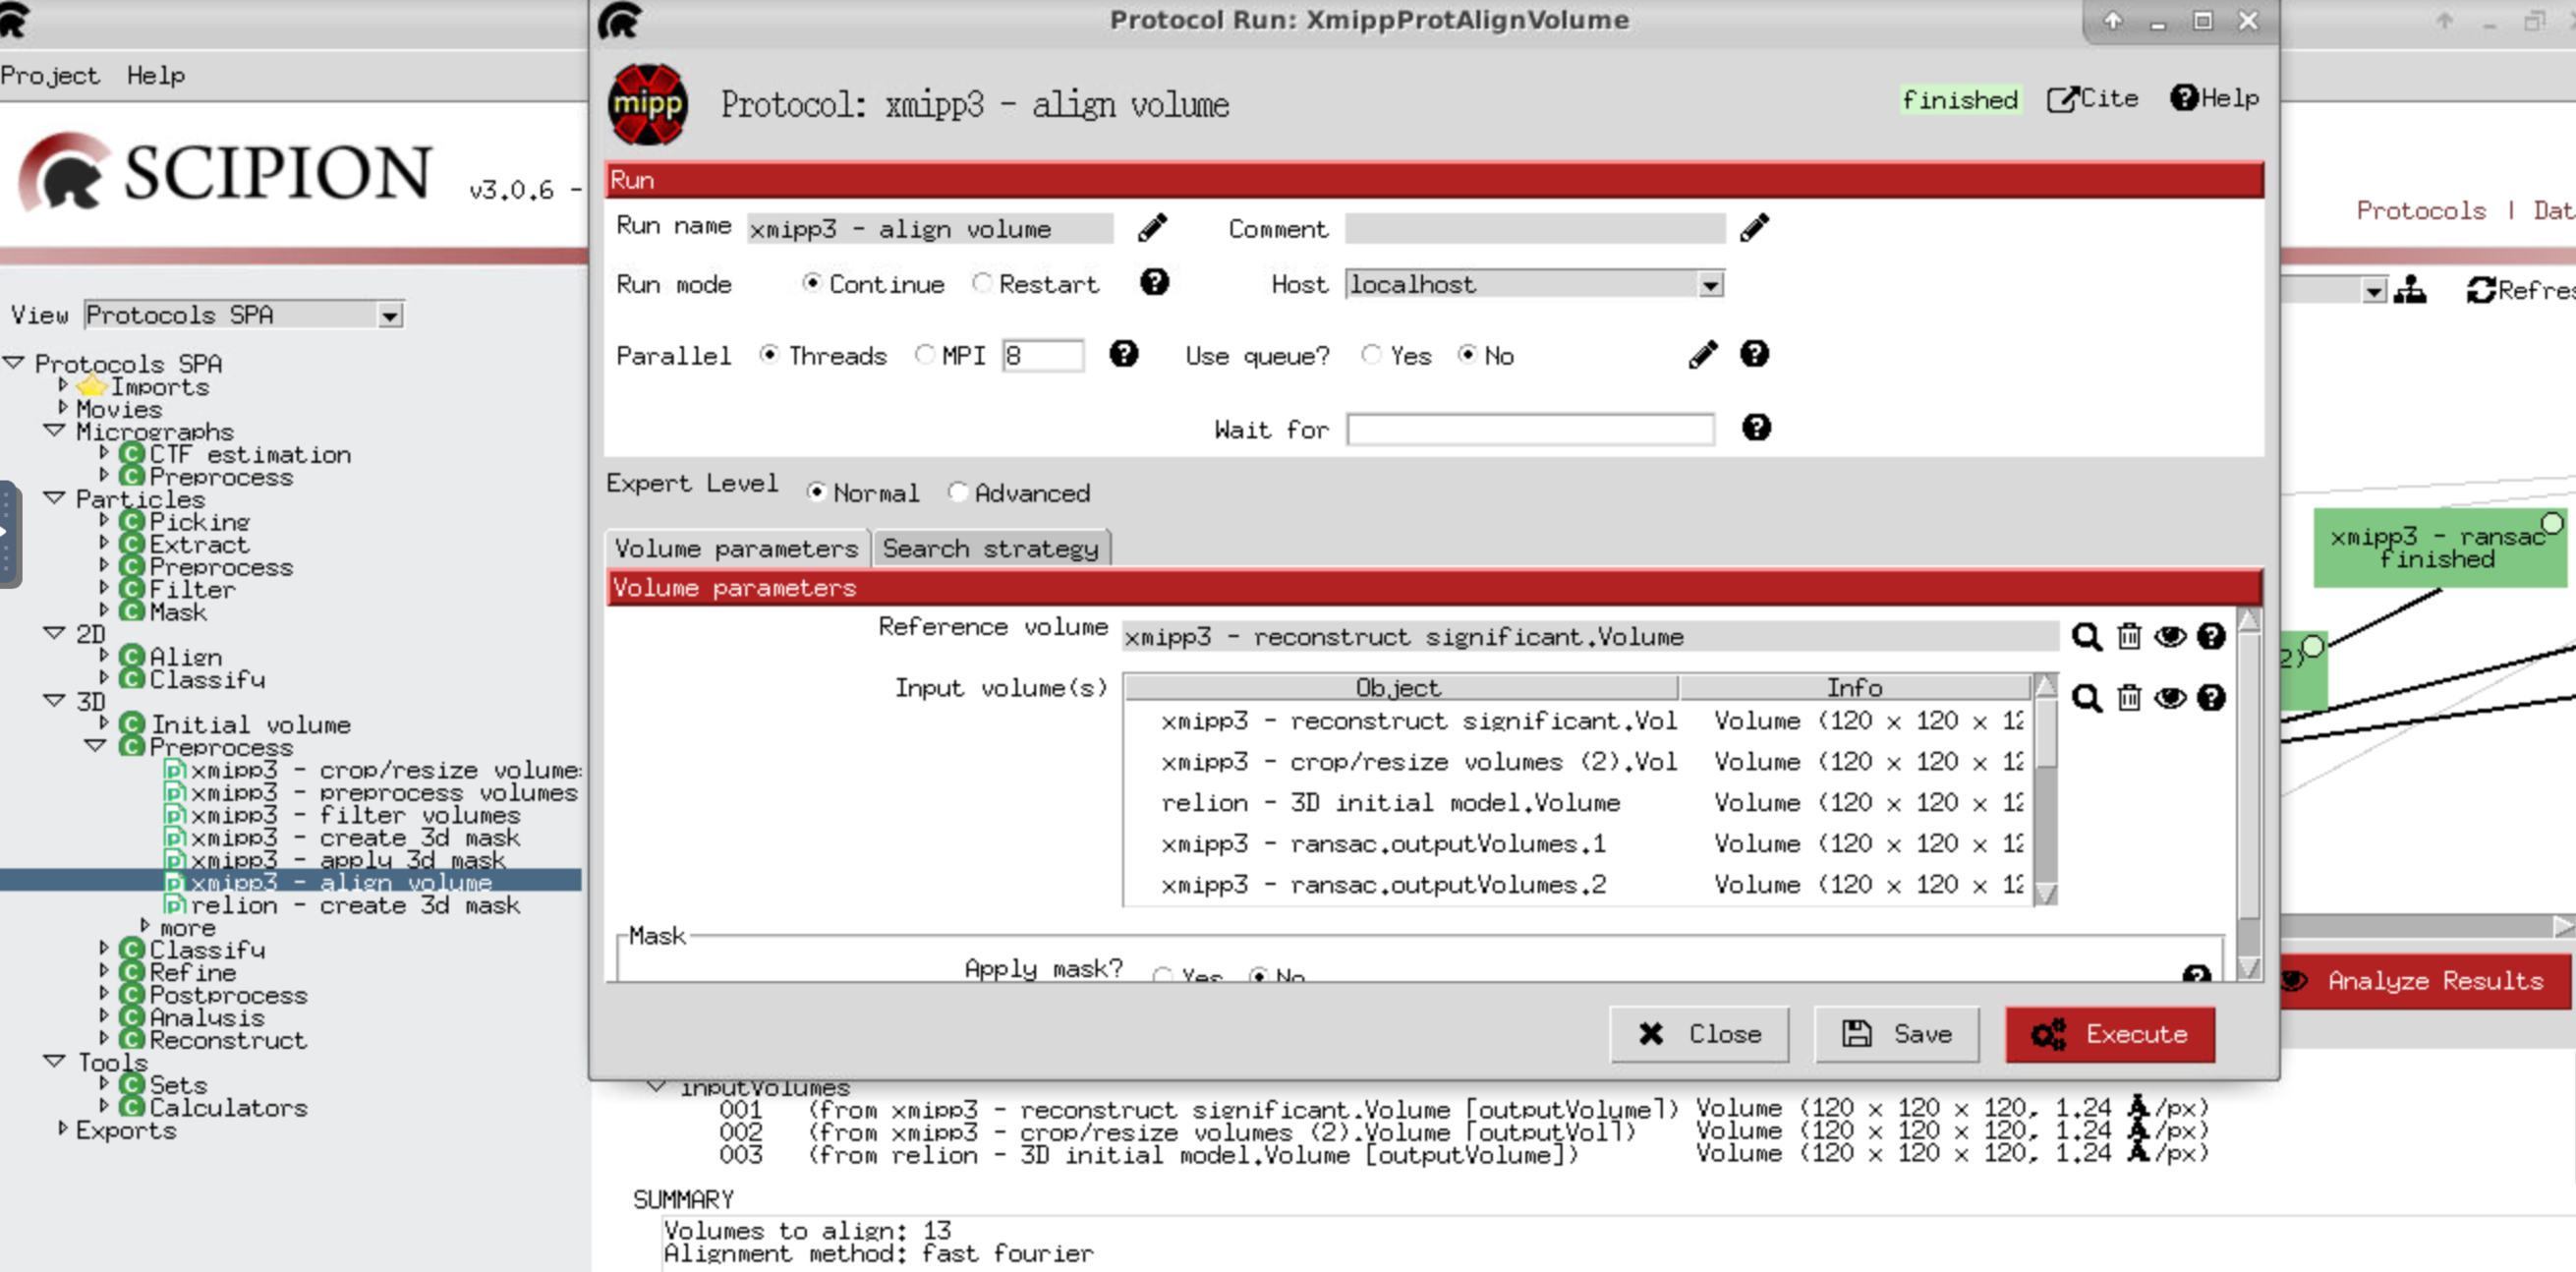
\includegraphics[width=0.95\textwidth]
  {images/8f_xmipp3_AlignVol.pdf}
  \caption{Completing the params for protocol \scommand{xmipp3-align volume}.}
  \label{fig:align_volume}
  \end{figure}
  
A new set of 13 volumes has been created keeping the same size and sampling rate shown by the initial particles. These volumes can be visualized by pressing \scommand{Analyze Results}.\\

Next, in order to have only one initial volume partially refined against the selected set of particles, we use the protocol \scommand{xmipp3-swarm consensus} (\ffigure{fig:swarn_consensus}). The inputs of this protocol are the set of 13 maps and the set of 3,491 $Relion$ extracted particles, previously generated. In this case, maps and particles have the same size and sampling rate. The program try to optimize the correlation between the swarm of volumes and the set of particles. Only a fraction of the particles are used to update this stochastic maximization.

\begin{figure}[H]
  \centering
  \captionsetup{width=.8\linewidth} 
  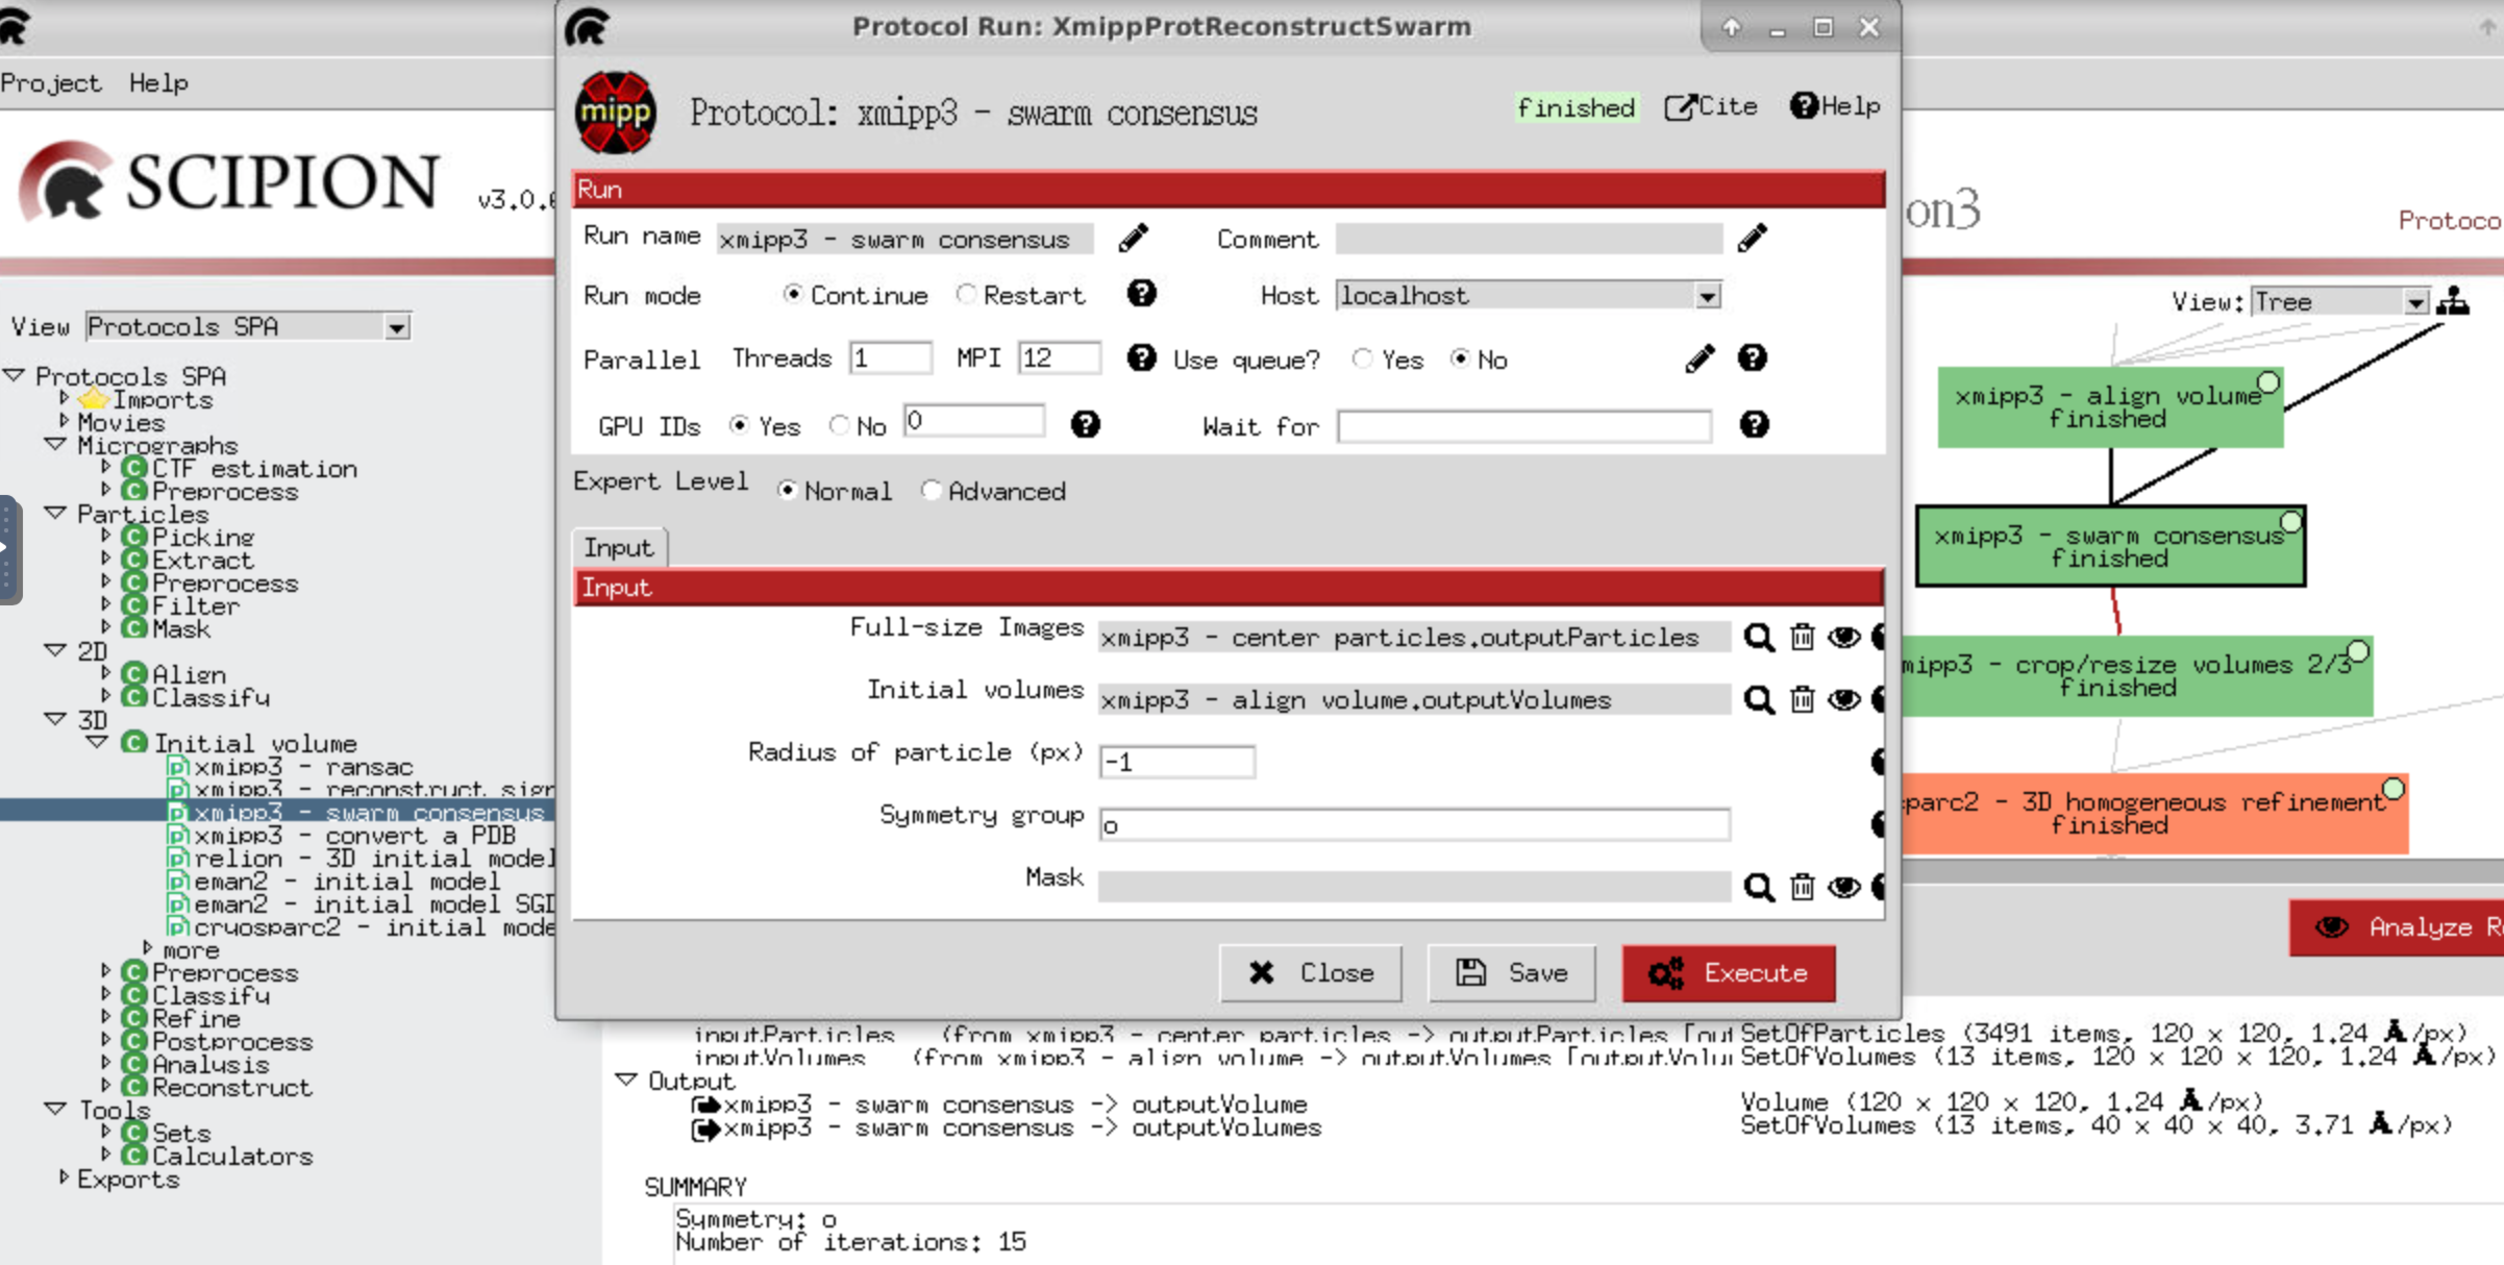
\includegraphics[width=0.95\textwidth]
  {images/8g_xmipp3_swarnconsensus.pdf}
  \caption{Completing in the params of the protocol \scommand{xmipp3-swarm consensus}.}
  \label{fig:swarn_consensus}
  \end{figure}
  
After 15 iterations, this protocol generates two outputs, a downsampled set of volumes and a volume with the size and sampling rate of the inputs. However the \scommand{xmipp3-swarm consensus} produced a volume that is of a difference pixel size than the extracted particles from the step before, therefore we need to apply \scommand{xmipp3-crop/resize volumes} (\ffigure{fig:crop_resize_volumes2}) to obtain the same dimensions. As input, select the output volume\/s of the previous protocols, \ttt{Sampling Rate} for \ttt{Resize option}, and 250 px as \ttt{Window size}.

\begin{figure}[H]
  \centering
  \captionsetup{width=.8\linewidth} 
  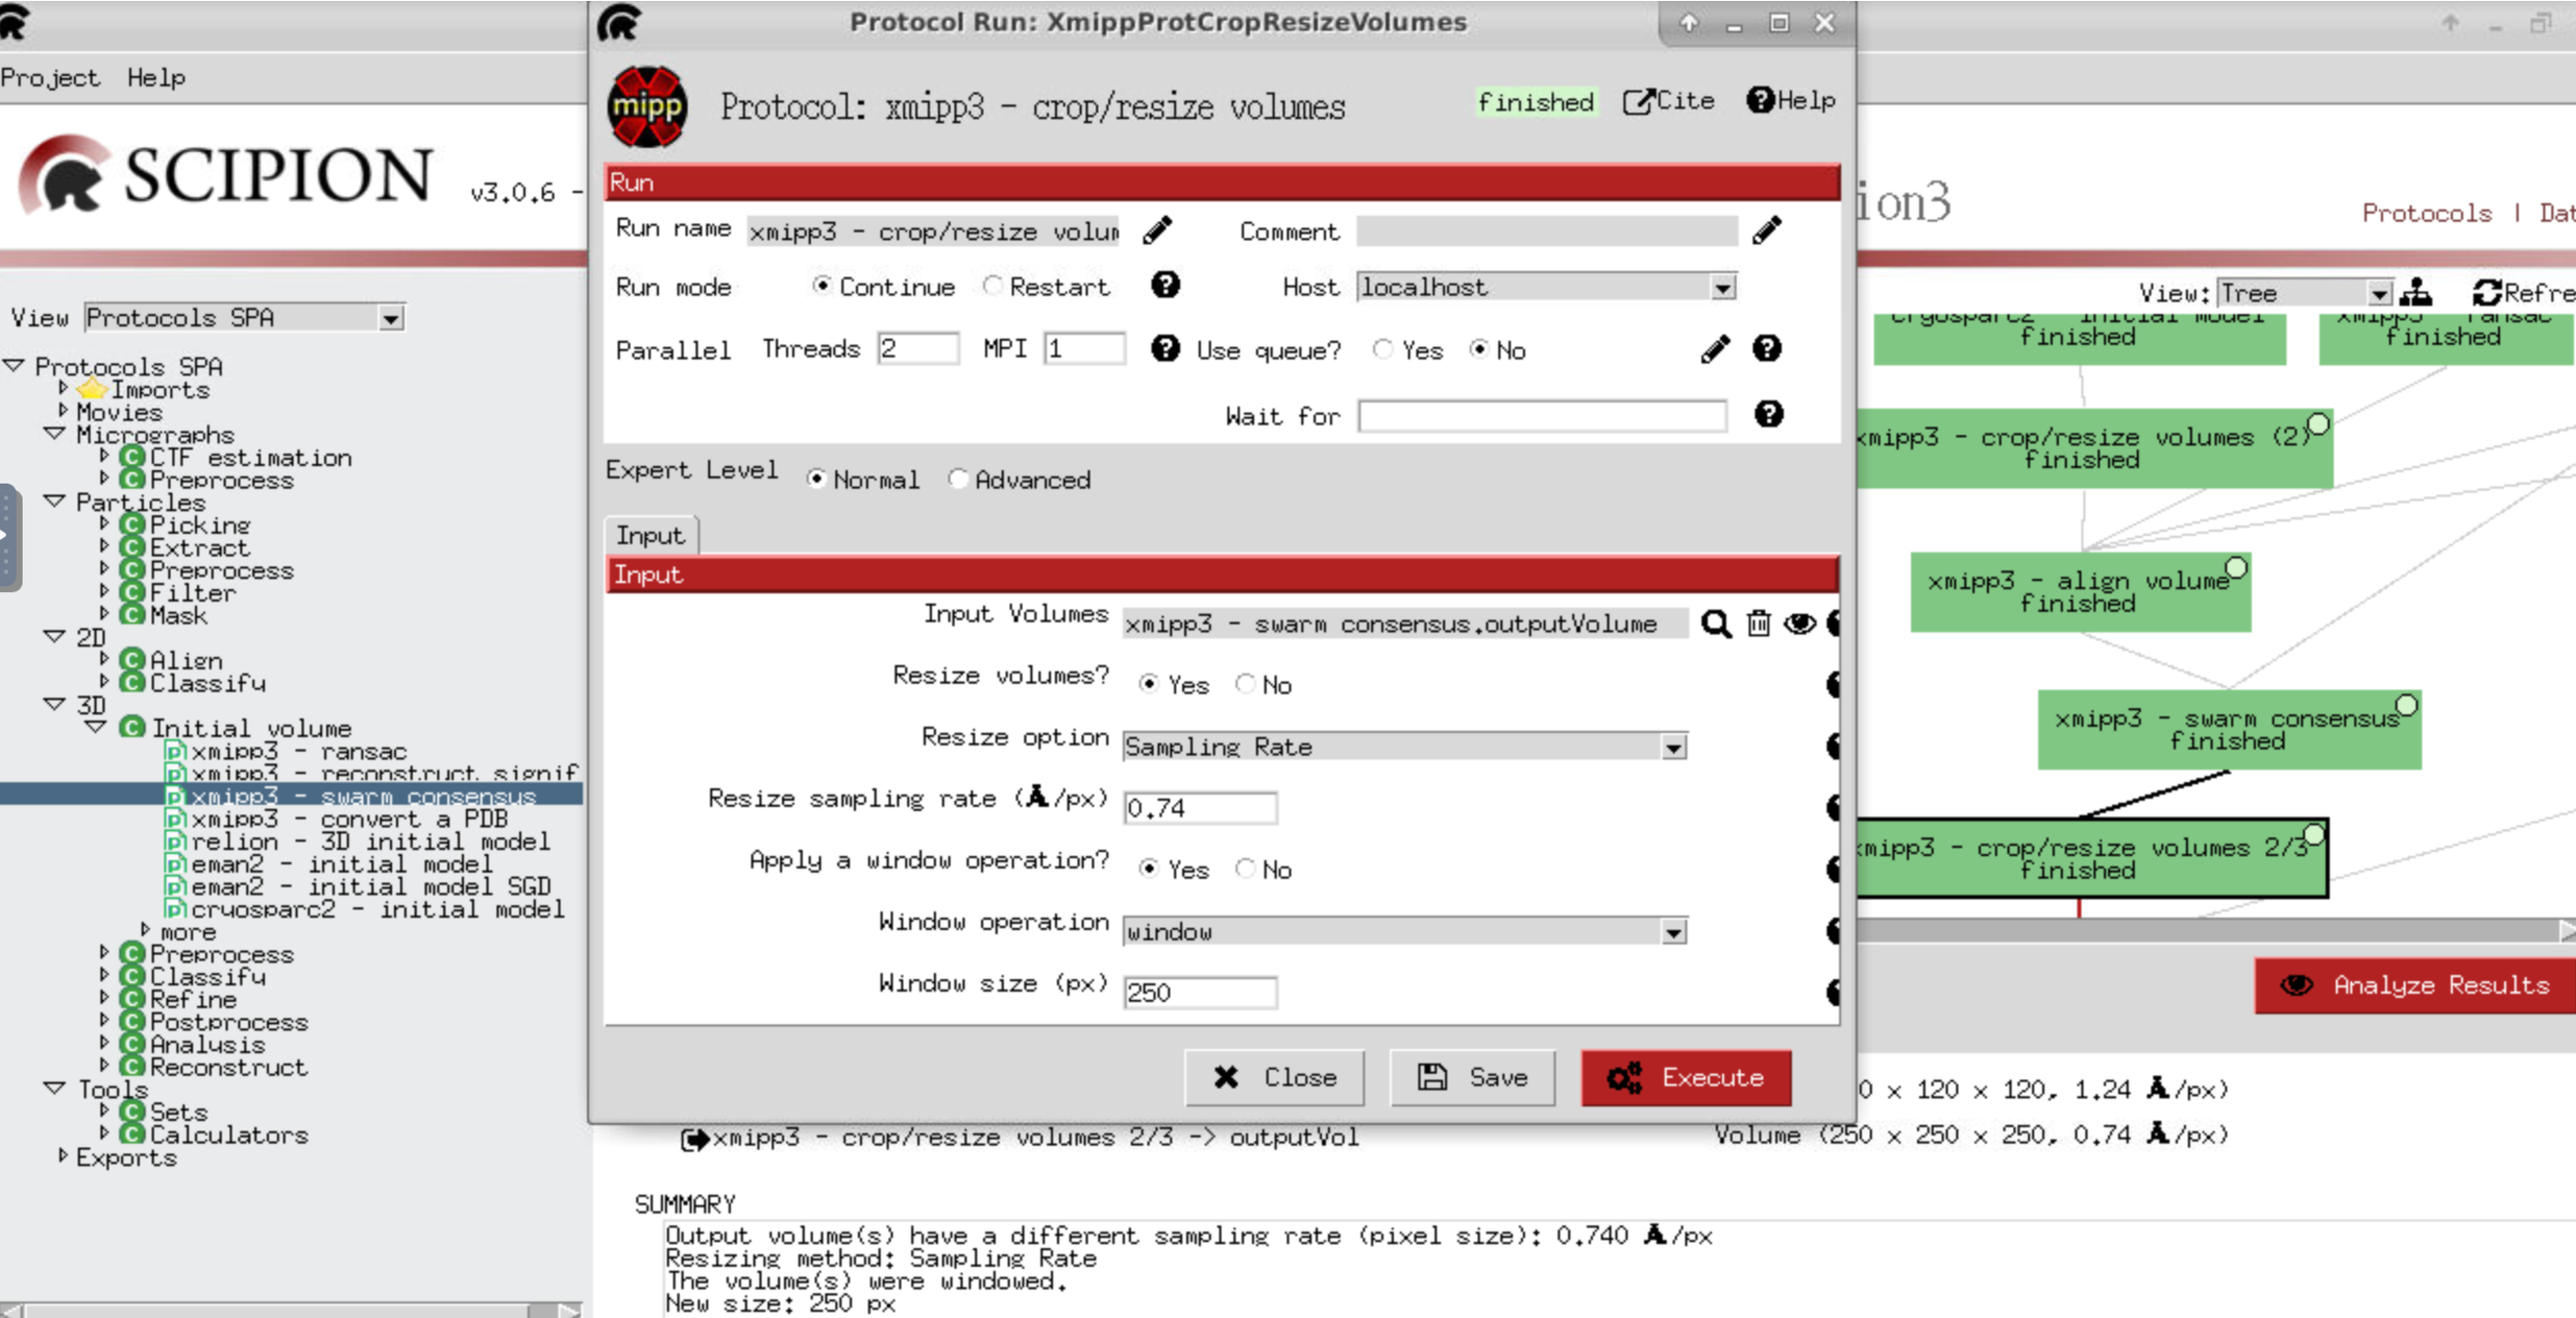
\includegraphics[width=0.95\textwidth]
  {images/8h_xmipp3_crop_resize.pdf}
  \caption{Params of protocol \scommand{xmipp3-crop/resize volumes}.}
  \label{fig:crop_resize_volumes2}
  \end{figure}

 At this point, we have an initial volume that has been chosen from many proposed algorithms and from the previous step we have extracted the set of particles that are not duplicated and had pass through all the picking and 2D filtering process and both of the same dimensions. These will be used for the next step in the workflow of 3D Classification and Refinement.\\
 
   For more information: 
\begin{itemize}
   \item \textbf{Video tutorial}: \url{https://www.youtube.com/watch?v=ppZXg4B7Q7U&list=PLQjWIcrmtc4JjyC-_BM99_XW-VsDa4_i3&index=28}.
   \item \textbf{Theoretical lecture}: \url{https://www.youtube.com/watch?v=jzEXzW3VB1w&list=PLQjWIcrmtc4JjyC-_BM99_XW-VsDa4_i3&index=34}.
  \end{itemize}

